\chapter{Neuroprotective effects of tibolone during astrocytic metabolic inflammation: a network based approach}
\section*{Abstract:}d
\section{Introduction}
\section{Material and Methods}
\subsection{Tissue Specific Model Construction}
The tissue specific model construction process started with the identification of all enzyme‐coding genes expressed over the mean in at least 50\% of samples for healthy human astrocytes indexed in the GEO database \cite{Edgar2002} as GSE73721 \citep{Zhang2016}. Gene identificators convertion from GeneCards\cite{rebhan1997genecards} to ENTREZ \cite{maglott2005entrez} was performed throught `UniProt.ws' R Package \cite{Carlson2016}. Reactions associated with the identified genes were mapped from the Human Genome Scale  Metabolic Reconstruction RECON 2.04 downloaded from the VMH Lab (https://vmh.uni.lu) \cite{thiele2013community}. The R package `g2f' \cite{G2F} was used to identify and fill the gaps using all no gene associated reactions included in RECON 2.04, as well as to identify and remove all blocked reactions  from the reconstruction. All reactions involved in the conversion of extracellular glutamate, glycine, cysteine and glucose to extracellular glutamine, glycine, serine-D, reduced glutathione, lactate and ATP respectively were added. Exchange reactions were limited to components of the Dulbecco's Modified Eagle Medium (DMEM) as input and gliotransmitters () as output. Finally, syntax, mass-charge validation and creation of SBML files were carried out through the `minval' R Package \cite{MINVAL}. Reaction limits (upper and lower bounds) were constrained proportional to the mean gene expression reported for genes included in Gene-Protein-Reaction (GPR) \cite{Thiele2010} associated to each reaction in samples of 47 to 63 years old using `exp2flux' R package \cite{EXP2FLUX}. All analysis were done by the `sybil' \cite{Gelius-Dietrich2013} R Package running under R 3.3.1 \cite{RCoreTeam2016}.
\subsection{Flux Balance Analysis}
Flux Balance Analysis (FBA) is a linear optimization method for simulating metabolism that allows to identify the set of reactions involved in the production of a biological response within a metabolic model \cite{Orth2010}. The metabolic reactions are represented internally as a stoichiometric matrix ($S$), of size $m * n$, where $m$ represents the compounds and $n$ the reactions; the entries in the matrix are the stoichiometric coefficients of the metabolites participating in a reaction \cite{Raman2009}. The flux through all of the reactions in a network is represented by the vector $v$, which has a length of $n$. The concentrations of all metabolites are represented by the vector $x$, with length $m$. The systems of mass balance equations at steady state, $\dfrac{d_{x}}{d_{t}}=0$ or $S * v = 0$. FBA seeks to maximize or minimize an objective function which can be any linear combination fluxes, to obtain a flux for each reaction, indicating how much each reaction contributes to the objective function \cite{Orth2010}. FBA for healthy, inflammated and medicated scenarios was resolved using GLPK 4.60, setting the generic human biomass reaction included in RECON 2.04 and each one of reactions described in table \ref{OF} as objective functions. Models were analyzed by comparing fluxes between scenarios, metabolites production rate and sensibility analysis.

\begin{table}[h]
\caption{Objective functions used to evaluate astrocytes metabolic capabilities}
\label{OF}
\begin{center}
\footnotesize{
\begin{tabular}{rlp{6cm}}
\hline
ID & FORMULA REACTION & DESCRIPTION \\
\hline
\hline
Glu2Gln & 1 glu\_L[e] $\Rightarrow$ 1 gln\_L[e] & Glutamate - Glutamine Cycle \\
Gly2SerD & 1 gly[e] $\Rightarrow$ 1 ser\_D[e] & Glycine to Serine conversion\\
Glc2Lac & 1 glc\_D[e] $\Rightarrow$ 2 lac\_L[e]& Lactate production from Glucose \\
Glc2ATP & 1 glc\_D[e] $\Rightarrow$ 36 atp[e] & ATP production from Glucose \\
Cys2GTHRD&1 cys\_L[e] + 1 glu\_L[c] + 1 gly[c] $\Rightarrow$ 1 gthrd[e]& Catch of Cysteine to produce reduced Glutathione \\
\hline
\end{tabular}}
\end{center}
\end{table} 
\subsection{Inflammated Scenario}
Inflammated Scenario was defined as an optimized model where uptake of palmitate was forced to be stable in the mean of the half maximal inhibitory concentration (IC50) value for all objective functions included in table \ref{OF}. IC50 values were calculated through a robutness analysis performed using uptake of palmitate (`EX\_hdca(e)' in RECON 2.04) as control reaction and a 1000 points in the range from 0 to 1 mMgDW$^{-1}$h$^{-1}$ for each objective function. Uptake value were each objective function reached IC50 was selected and subsequently averaged.
\subsection{Medicated Scenario}
\section{Results}
\begin{figure}[h]
\begin{center}
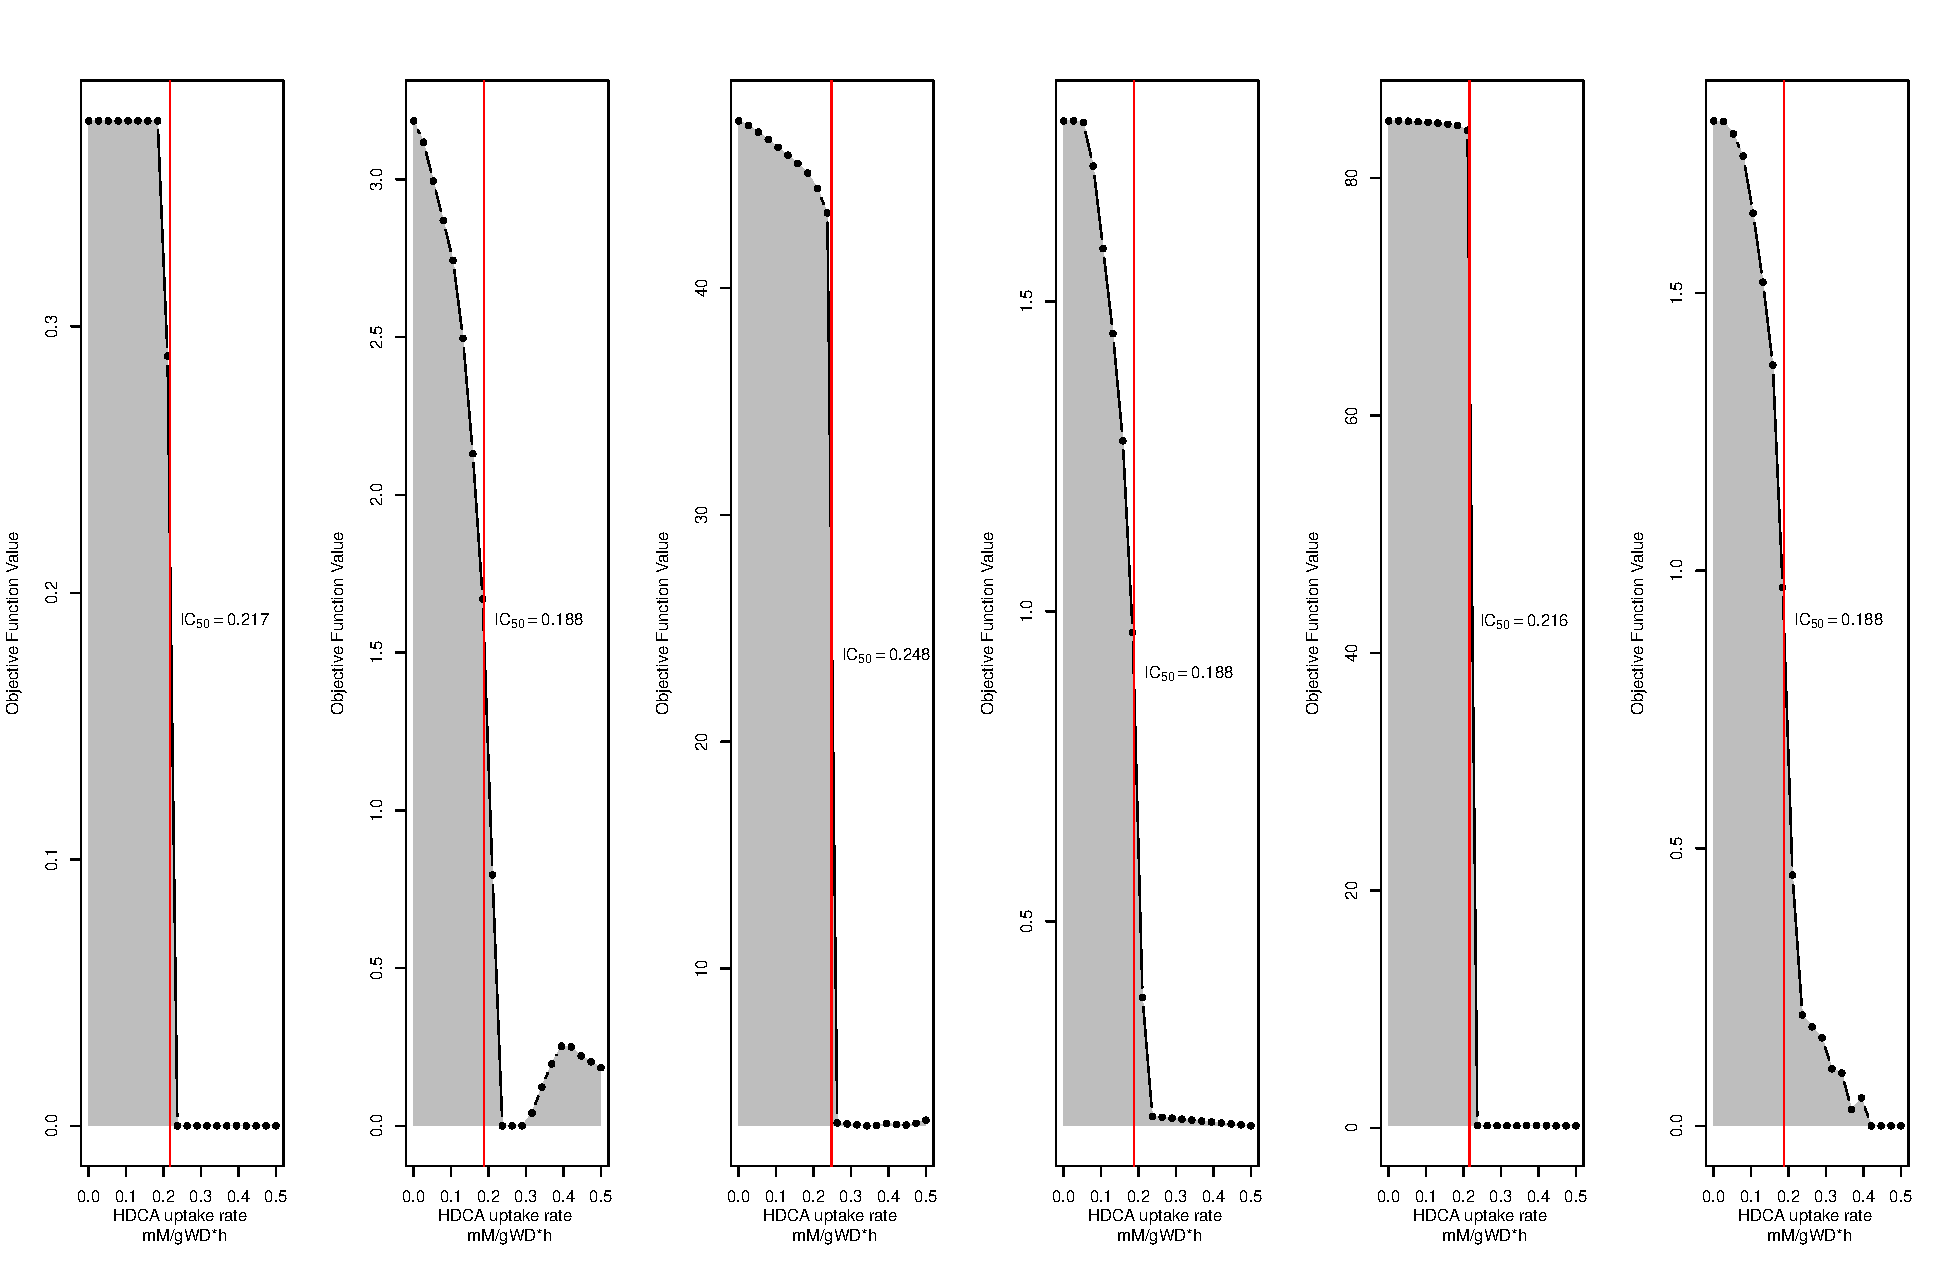
\includegraphics[width=\textwidth]{neuroprotective/IC50}
\end{center}
\caption{•}
\end{figure}
\begin{figure}[h]
\begin{center}
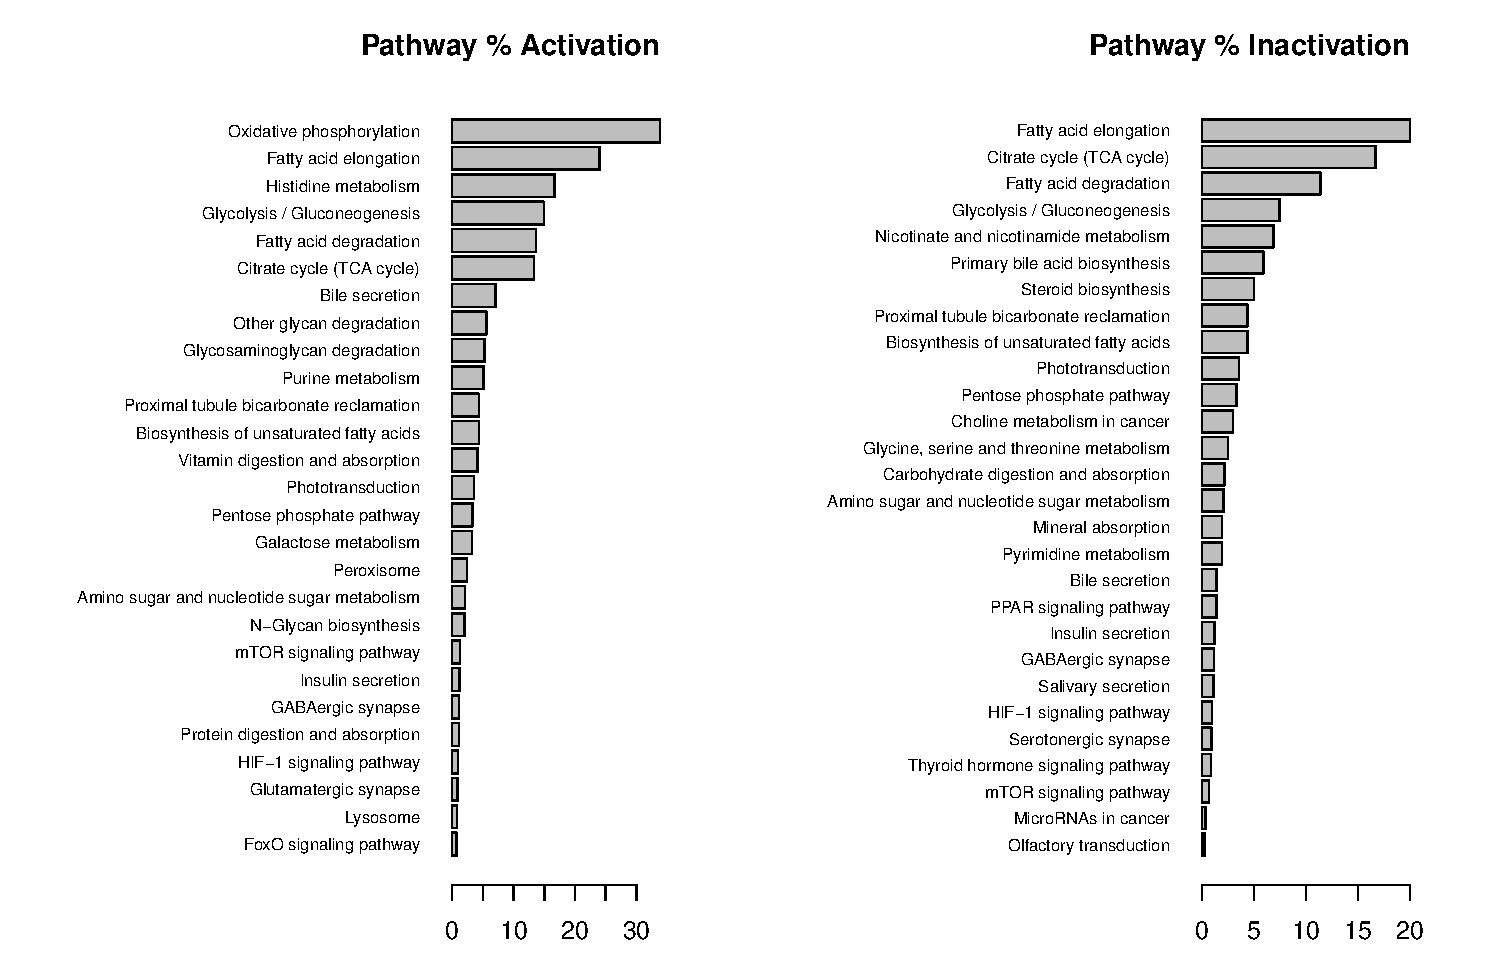
\includegraphics[width=\textwidth]{neuroprotective/Healthy2Inflammated}
\end{center}
\caption{•}
\end{figure}
\begin{figure}[h]
\begin{center}
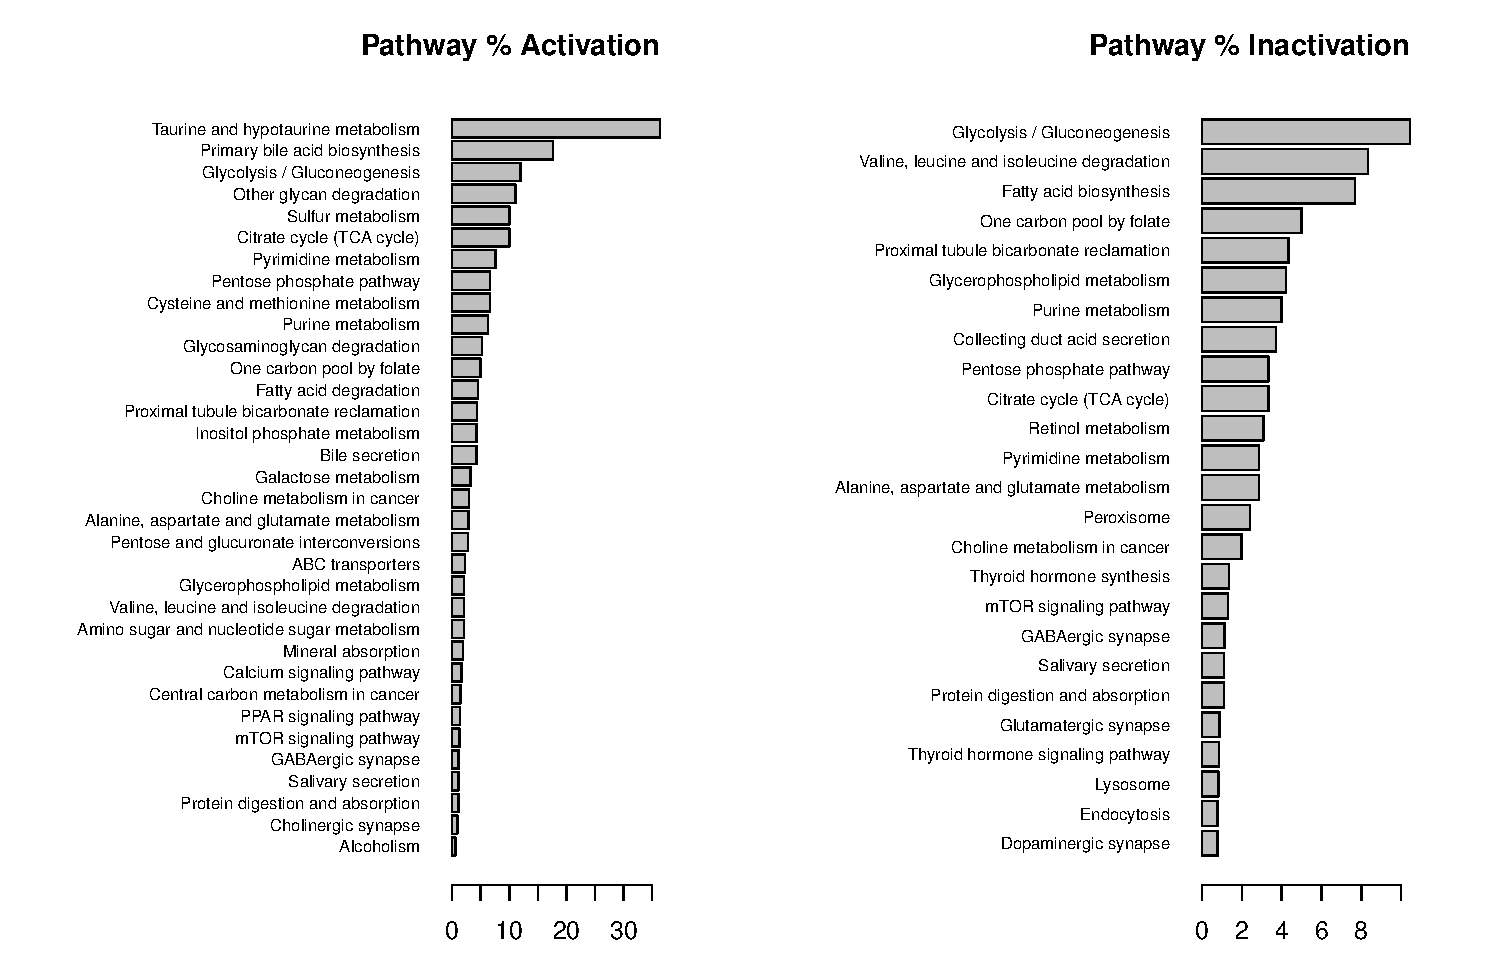
\includegraphics[width=\textwidth]{neuroprotective/Inflammated2Tibolone}
\end{center}
\caption{•}
\end{figure}
\section{Conclusion}
\section{Bibliography}

